%%%%%%%%%%%%%%%%%%%%%%%%%%%%%%%%%%%%%%%%%%%%%%
%                insertmeeting
% 1) Title (something creative & funny?)
% 2) Date (MM/DD/YYYY)
% 3) Location (ex. Hagerty High School)
% 4) People/Committees Present 
% 5) Picture 
% 6) Start Time & Stop Time (ex. 12:30AM to 4:30PM)
%%%%%%%%%%%%%%%%%%%%%%%%%%%%%%%%%%%%%%%%%%%%%%
\insertmeeting 
	{Front Wheel Fixes} 
	{10/20/21}
	{Hagerty High School}
	{Anouska, James, Nathan, Ritam, Samantha}
	{Images/RobotPics/robot.jpg}
	{1:30 - 4:30}
	
\hhscommittee{Hardware}
\noindent\hfil\rule{\textwidth}{.4pt}\hfil
\subsubsection*{Goals}
\begin{itemize}
    \item Redesign front wheel to allow for odometry 

\end{itemize} 

\noindent\hfil\rule{\textwidth}{.4pt}\hfil

\subsubsection*{Accomplishments}
As the robot’s hardware is advancing steadily, we have started thinking about how to davance it’s software, and one of the biggest ways to elevate our software game is to use odometry. Odometry is a type of localization that uses dead wheels attached to encoders to find the field position of the robot. Although there is a well tested and formulated version of odometry for normal drivetrain designs like tank and mecanum drive, our car drive works differently, meaning we will have to come up with all of the hardware and software ourselves. After talking with software about the best route to take for odometry, we came up with the idea of tracking the robots movements from the front wheel. We will have one encoder attached to the top to read how far to the left and right the front wheel is facing and another attached to the shaft of the front wheel to tell how far it has rotated. Using this information, the software committee can use inverse kinematics to figure out and control the robots position on the field at all times. For now, we need to redesign the front wheel to fit all of the encoders. Going into cad, we started adding a place onto the fork where an encoder can attach to read the rotations of the front wheel (Figure \ref{fig:pic1}). For this odometer we used a cui device's AMT-103 encoder for its small profile, which is important for the small space that it needs to fit into next to the wheel The next odometer will be a rev throughbore encoder placed above the front wheel, reading the direction the robot is facing (Figure \ref{fig:pic2}). By doing this, we can translate the readings from these encoders to track exactly where the robot is on the field (Figure \ref{fig:pic3}). 

 

\begin{figure}[ht]
\centering
\begin{minipage}[b]{.48\textwidth}
  \centering
  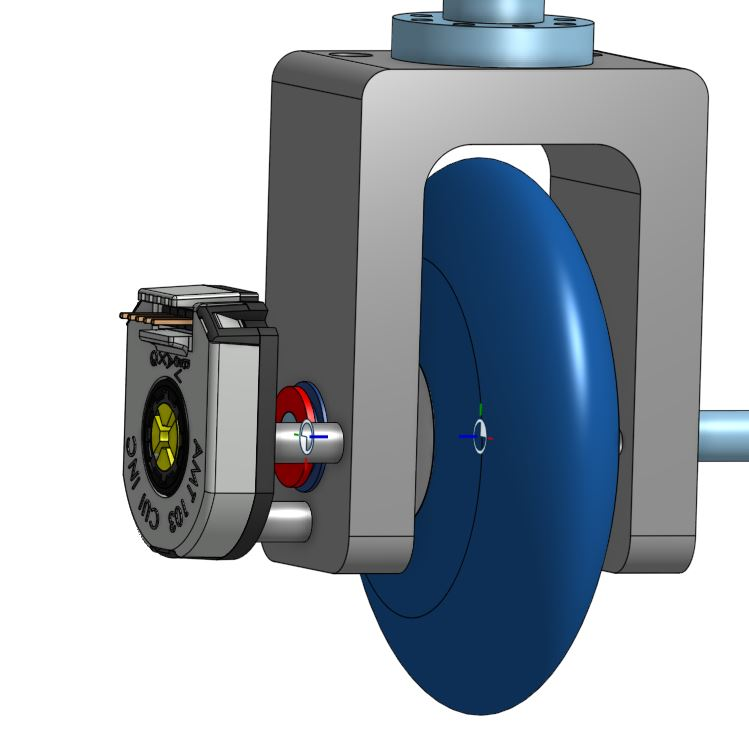
\includegraphics[width=0.95\textwidth]{Meetings/October/10-20-21/10-20-21_CAD_Figure1 - Nathan Forrer.JPG}
  \caption{The fork for an encoder.}
  \label{fig:pic1}
\end{minipage}%
\hfill%
\begin{minipage}[b]{.48\textwidth}
  \centering
  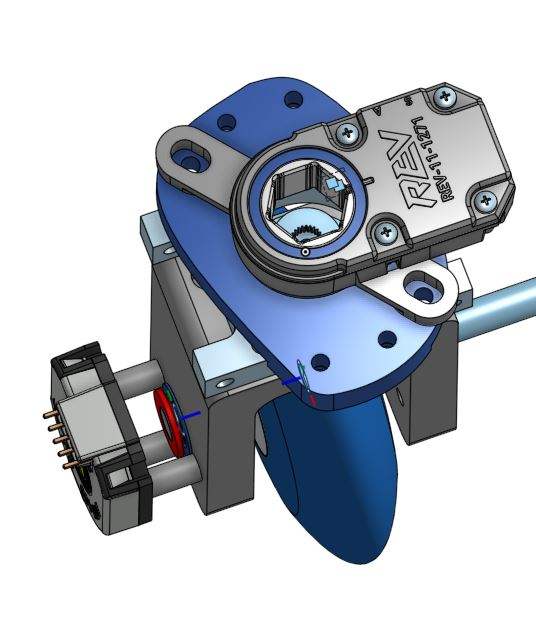
\includegraphics[width=0.95\textwidth]{Meetings/October/10-20-21/10-20-21_CAD_Figure2 - Nathan Forrer.JPG}
  \caption{Our REV encoder to read steering angle.}
  \label{fig:pic2}
\end{minipage}
\end{figure}

\begin{figure}[htp]
\centering
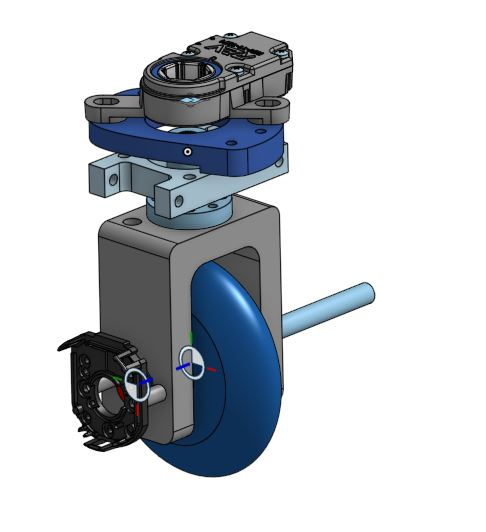
\includegraphics[width=0.95\textwidth, angle=0]{Meetings/October/10-20-21/10-20-21_CAD_Figure3 - Nathan Forrer.JPG}
\caption{The final assembly.}
\label{fig:pic3}
\end{figure}

\whatsnext{
\begin{itemize}
    \item Finish drivetrain
    \item Attach front wheel

\end{itemize} 
}

